\documentclass[msc]{cls_bst/cls_file_ufam_v2}

% PARA DEFESA DE DISSERTAÇÃO DE MESTRADO USE   : msc
% PARA DEFESA DE QUALIFICAÇÃO DE MESTRADO USE  : mscexam

% PARA DEFESA DE TESE DE DOUTORADO USE         : dsc
% PARA DEFESA DE QUALIFICAÇÃO DE DOUTORADO USE : dscexam



%% pacotes e sets
%\usepackage{lscape}
\usepackage{pdflscape}
\usepackage[english,brazil]{babel}
\usepackage[utf8]{inputenc}
\usepackage[T1]{fontenc}
\usepackage{indentfirst}
\usepackage{fancyhdr}
\usepackage{url}
\usepackage{cite}
\usepackage{epstopdf}
%\usepackage{subfigure}
\usepackage{subcaption} 
\usepackage{epsfig}
\usepackage{longtable}
\usepackage{setspace}
\usepackage{rotating}
\usepackage{graphicx}
\usepackage{dsfont}
\usepackage{enumerate}
\usepackage{amsmath}
\usepackage{color}
\usepackage{bbm}
\usepackage{amssymb}
\usepackage[final]{pdfpages}
%\usepackage[number=none]{glossary}
\usepackage{glossaries}
%\usepackage[acronym]{glossaries}
\usepackage{float}
\usepackage{multirow,colortbl,array}
\usepackage{hhline}
\usepackage{makecell}
\usepackage{nomencl}
\usepackage[mathletters]{ucs}
\usepackage{comment}
\usepackage[dvipsnames]{xcolor}
\usepackage{pdfpages}
%% pacote para hyperlinks

\usepackage{amsmath}
\usepackage{amsfonts}
\usepackage{algorithm}
\usepackage{algpseudocode}
\usepackage{geometry}
\geometry{margin=1in}

\usepackage[
    colorlinks=true,  % Ativa links coloridos em vez de caixas
    linkcolor=blue,   % Cor dos links internos (ex: sumário)
    citecolor=red,    % Cor dos links de citação
    urlcolor=magenta,  % Cor dos links externos (URLs)
     pagebackref=true,
]{hyperref}



\makenomenclature

\setcounter{secnumdepth}{3}
\setcounter{tocdepth}{2} %where 3
\setcounter{chapter}{0}
\setlength{\parindent}{1.25cm}
%%%%%%%%%%%%%%%%%%%%%%%%%%%%%%%%%%%%%%%%%%%%%%%%%%%%%%%%%%

%% LISTA DE SIGLAS
\makeglossaries
\newacronym{qnn}{QNN}{Quantized Neural Network}
\newacronym{dnn}{DNN}{Deep Neural Network}
\newacronym{relu}{ReLU}{Rectified Linear Unit}
\newacronym{bnn}{BNN}{Binary Neural Network}
\newacronym{smt}{SMT}{Satisfiability Modulo Theories}
\newacronym{milp}{MILP}{Mixed-Integer Linear Programming}
\newacronym{nn}{NN}{Neural Network}
\newacronym{ptq}{PTQ}{Post-Training Quantization}
\newacronym{qat}{QAT}{Quantization-Aware Training}

\begin{document}

%\pagenumbering{Roman}
%\pagenumbering{Arabic}


%%%%%%%%%%%%%%%%%%%%%%%%%%%%%%%%%%%%%%%%%%%%%%%%%%%%%%%%%%
  \title{Formal Synthesis of Quantized Neural Networks: An SMT-Based Approach for Bit-Precise Verification}
  
  \foreigntitle{Formal Synthesis of Quantized Neural Networks: An SMT-Based Approach for Bit-Precise Verification}
  
  \author{João Victor}{Lima de Souza}
  
  \advisor{Prof.}{Lucas}{Cordeiro}{D.Sc.}
  %\coadvisor{Prof.}{André Luiz}{Aguiar da Costa}{D.Sc.}
  % \socoadvisor{Prof.}{André Luiz}{Aguiar da Costa}{D.Sc.}
  \examiner{Prof.}{}{D.Sc.}
  \examiner{Prof.}{}{D.Sc.}
   \department{MEE} %nao mudar---- formato para mestrado
  %\department{EE}
  \date{03}{2025}

% \keyword{Classificação Automática de Modulação}
% \keyword{Comunicações Ópticas}

\maketitle

\frontmatter

%inserir linha em cima da pagina ---------
\thispagestyle{empty}
%-----------------------------------------

\dedication{Gostaria de expressar minha gratidão...}

\chapter*{Agradecimentos}
Expresso minha profunda gratidão...

\begin{abstract}


\textbf{Palavras-chave:} Classificação Automática de Modulação, Redes Ópticas, \textit{Random Forest}, \textit{Perceptron} Multicamada.
\end{abstract}

\begin{foreignabstract}


\textbf{Keywords:} Automatic Modulation Classification, Optical Networks, Random Forest, Multilayer Perceptron.
\end{foreignabstract}
%inserir linha em cima da pagina --------------------------------------------------------
   \pagestyle{plain}
   \lhead[\fancyplain{}{\bfseries\tiny\thepage}]{\fancyplain{}{\bfseries\tiny\rightmark}}
   \rhead[\fancyplain{}{\bfseries\tiny\leftmark}]{}
%----------------------------------------------------------------------------------------

  \tableofcontents
  \listoffigures
  \listoftables
\renewcommand{\glossaryname}{Lista de Siglas}
\printglossaries
\mainmatter

\begin{comment}
    

    Nessa paper vamos focar na verificação de redes Redes Neurais Convulacionais Quantizadas (QCNNs) lidando como o problema da equivalência de código entre a função original e a função quantizadas.

    O objetivo do paper é mostrar que o método de verificação BMC com SMT pode ser usado para garantir a confiabilidade de QCNNs no processamento de imagens em sistemas de menor potência computacional.
    
    Existem trabalhos que usam SMT para verificar o modelo matemático, mas como mostrado por \cite{cordeiro2025neuralnetworkverificationprogramming} ele deve ser tratado como um programa de verificação de programa.

    Verificar no BMC
    --multi-property
    --parallel-solving
    --smt-symex-guard


\end{comment}


\chapter{Introduction}\label{cap:intro}

%%% First talk about the advances of AI in everyday life 
%%% Then talk about how much have AI models grown 
%%% Use present tense when talking about this dissertation and past tense when talking about past works.

\section{Background}\label{sec:background}
From the first Artificial Neural Network (ANN) models such as Perceptron, which was proposed in 1958 \cite{Rosenblatt1958}, to the current state-of-the-art models like GPT-4 \cite{OpenAI2023GPT4}, ANN has become a transformative force across various sectors. It is used in healthcare for diagnostics such as Parkison disease detection \cite{Luo2025Efficient}, in autonomous vehicles for safety features using Convolutional neural networks (CNNs) to detect driver distraction in real time \cite{Lei2025An}, and in finance for fraud detection by analyzing transaction patterns using advanced machine learning algorithms \cite{Zhu2024A}. These examples illustrate the profound impact of these models on our daily lives, improving efficiency, safety, and decision-making processes. 

%%% Then talk about the usage of AI in embbeded fields, such as smartphones and IoT devices
However, these state-of-the-art ANNs are often too large and complex to be deployed on devices with limited resources, such as smartphones and IoT devices \cite{Zhu2020Survey}. The computational demands of these models can lead to significant latency and energy consumption, making them impractical for real-time applications in resource-constrained environments.


\begin{comment}
    %%%% These papers talk using quantization to reduce the floating point precision to fixed point precision.
    (JACOB et al., 2017;  LIN; TALATHI; ANNAPUREDDY, 2016)
    %%%% These techniques reduce network size and computational requirements
    (HAN; MAO; DALLY, 2016; NAGEL et al.,  2021)
    %%% However it lead to a trade-off between model size and accuracy
    (JACOB et al., 2017; HUBARA et  al., 2017)
\end{comment}

%%% Here we will talk about the quantization problem of neural networks, the use of SMT solvers to solve combinatorial problems, and the motivation for this work.

To address these challenges, quantization techniques are commonly used to reduce the size of models \cite{Zhu2016Trained, Zhu2020Survey}. It involves reducing the precision of the model's weights, activations, and bias, which can lead to a significant reduction in memory usage and computational requirements. However, this process often results in a trade-off between model size and accuracy, as lower precision can lead to degration of performance and therefore its accuracy \cite{Zhou2017Incremental}.

In works such as \cite{cai2025certified}, the authors have highlighted two critical safety properties of QNNs: robustness and backdoor-freeness. The robustness would refer to the model's ability to resist small input perturbations that change the classification, while the former refers to the ability of not having backdoors, which could be intentionally explored with malicious intent. These properties are of utmost importance to ensure the reliablity and safety of QNNs.


\section{Motivation}\label{sec:motivation}

%% Vms abordar a motivação do uso de quantização e a necessidade de verificar a integridade dos modelos quantizados.


Thus, the need to ensure the reliability of ANN models after going through quantization is demonstrated since these models are being employed in critical applications, e.g., healthcare, autonomous vehicles, financial system fraud detection, among others \cite{OpenAI2023GPT4, Luo2025Efficient, Lei2025An, Zhu2024A}. In these scenarios, the models must not only be efficient to run on resource-constrained environments but also maintain their robustness and safety properties while keeping it's accuracy. 

% The process of quantization tries to mitigate the disadvantages of process, but fail. let's write about it.
Modern quantization techniques, such as those proposed by \cite{Zhu2020Survey, han2015deepcompression, han2020understanding, jacob2018quantization, Cai2020Certified, Zhou2017Incremental}, aim to reduce the loss of accuracy while minimizing the size of the model by employing a different set of strategies such as weight sharing, pruning, and factorization of low rank. However, these techniques often do not guarantee that the quantized model will retain its robustness or be backdoor-free.

In order to ensure that the quantization process does not compromise the model's performance, some verification techniques such as Formal Methods are employed. These methods can be used to verify the integrity of the quantized model by checking if the quantized model still meets the safety properties like the original model.
\begin{comment}
    
    %% We will talk about the need to verify the integrity of quantized neural networks, and how SMT solvers can be used to verify the integrity of these models.
    Therefore, it is essencial to have a robust mehtod to verify the integrity of QNNs, ensuring they still meet their requirements and perform securily to their intended tasks. 
    
    
    While quantization can make models more efficient, it is crucial to verify that the quantized model still meets the required performance standards. 
    
    Think of a scenario where a quantized model is embbeded in a medical device for a real-time diagnostics or a self-driving car where the most precision is required. In such cases, any degradation in model performance due to quantization is unacceptable. Therefore, given the important of these applications, it is essential to have a robust method for verifying the integrity of quantized models.
    
    ANN are widely used in various applications, but their computational and memory resource demands are high \cite{amir2021smt, han2020understanding, abdi2021counterexample, song2023qnnrepair}. Quantization is a crucial technique to mitigate this problem by reducing the bit-width (from 32-bit floating-point to 8-bit integers or even binary) used to represent weights, biases, and activations, making networks more efficient on embedded and low-power devices \cite{amir2021smt, han2020understanding,song2023qnnrepair, abdi2021counterexample, Cai2020Certified}.
    % This paragraph we will talk about other works that have verified the integrity of neural networks. Then we will talk about the use of MILP to verify preimage of neural networks and use it to verify the integrity of quantized neural networks. However, this approach does not verify using fixed-point precision like SMT solvers do.
\end{comment}
\section{Problem Statement}\label{sec:problem_statement}

%The formal method aims to address the implementation gap \cite{cordeiro2025neuralnetworkverificationprogramming}. 
Most formal verification techniques for neural networks (such as Reluplex and Marabou) assume that networks operate with real-number arithmetic \cite{katz2017reluplex,amir2021smt}. In contrast, actual hardware implementations use finite-precision arithmetic, such as low-precision floating-point or, more frequently, fixed-point \cite{han2020understanding}.

Furthermore, quantization, while beneficial for efficiency, can degrade accuracy and, more critically, compromise desired safety properties. Existing works on QNN verification generally focuses on post-hoc analyses; that is, they verify a network after it has been quantized \cite{eleftheriadis2022neuralnetworkequivalencechecking,song2023qnnrepair,katz2017reluplex,baranowski2020smt, Pulina2012Challenging, cordeiro2025neuralnetworkverificationprogramming} aiming to ensure that the quantization process does not introduce vulnerabilities or degrade of accuracy. However, these approaches do not guarantee the optimal quantization strategy unlinke the work of \cite{abdi2021counterexample,cai2025certified}, which proposes a framework to find a optimal bit-width for each layer of a QNN.

In contrast, the use of Mixed Integer Linear Programming (MILP) solvers has been proposed to verify the preimage of QNNs \cite{cai2025certified}. This approach allows for the verification of robustness and backdoor-freeness properties of QNNs. While having achieved promissing results in preserving these properties, it does not consider the fixed-point precision used in QNNs as done by \cite{baranowski2020smt}.

Since the verification problem in \cite{cai2025certified} uses MILP solvers, it does not formally incorporate the nuances of fixed-point arithmetic during verification. This work aims to fill this gap by integrating the SMT Theory of Fixed-Point Arithmetic, as formalized by \cite{baranowski2020smt}, into the preimage calculation and quantization process. This integration will allow the synthesis of quantization strategies that are certified for specific finite precision, ensuring that properties hold even with the effects of round and overflow.

\begin{comment}
    
    Several works have explored the verification of neural networks, particularly focusing on verification problem like a code problem \cite{cordeiro2025neuralnetworkverificationprogramming}. Some works like \cite{katz2017reluplex,katz2019marabou,abdi2021counterexample,song2023qnnrepair} use SMT solvers to verify the integrity of QNN by checking properties such as robustness\footnote{resistência a perturbações} and safety. However, these approuches typically do not scale well to large models and also do not take into account the fixed-point precision used in quantized models. In contrast, the use of MILP solvers has been proposed to verify the preimage of QNNs \cite{cai2025certified}. This approach allows for the verification of robustness and backdoor-freeness properties of QNNs. Though the work lacks to consider the fixed-point precision used in quantized models as done by \cite{baranowski2020smt}. It then lays the foundation for our work.
    
\end{comment}

\section{Objectives}\label{sec:objectives}

The goal of this work is to develop a end-to-end framework for the synthesis of quantization strategies that guarantee the preservation of robustness and backdoor-freeness properties after quantization, while directly addressing finite-precision arithmetic. This will differ form post-hoc approaches and quantization techniques that focus solely on accuracy as the primary goal will be to ensure a optimal quantization bit-width precision for each layer of the QNN. To formally achieve the proposed goal, the following specific objectives have been defined:

\begin{itemize}
    \item \textbf{Formalize the SMT Theory to encode Quantization Synthesis:} Integrate the SMT Theory into the preimage calculation and quantization process, allowing for the synthesis of quantization strategies that are certified for specific finite precision.
    \item \textbf{Adapt the MILP Formulation to SMT:} Adapt the Mixed-Integer Linear Programming (MILP) formulation used in \cite{cai2025certified} to a SMT formulation that reflects fixed-point operations, ensuring that the preimage calculation accounts for the effects of finite precision.
    \item \textbf{Validade Framework:} Validate the proposed framework by applying it to a set of NNs, demonstrating its effectiveness in synthesing quantization that preserve the desired properties.
    \item \textbf{Evaluate Performance:} Evaluate the performance of the proposed framework in terms of scalability and efficiency, comparing it with existing approaches. 
    
\end{itemize}

\begin{comment}
    
    
    This dissertation proposes the development of a framework for the certified synthesis of quantization strategies that guarantee the preservation of desired properties after quantization, directly addressing finite-precision arithmetic. This differs from post-hoc approaches and quantization techniques that focus solely on accuracy.

    \textbf{Synthesis of Quantization Strategies (Inspired by Quadapter):}
The work Quadapter is the first to propose the synthesis of certified quantization strategies \cite{Zhu2021Quadapter,Cai2020Certified}. Its central idea is to compute the preimage of each layer with respect to the desired output region and then identify the minimum bit-width for each layer, ensuring that the quantized layer's reachable region remains within that preimage.

This work would extend this line of research by focusing on the incorporation of fixed-precision arithmetic during the synthesis process. This is not the primary focus of Quadapter in its current state, which, while dealing with realistic quantization representations, does not yet formally incorporate the nuances of fixed-point arithmetic during verification.

\textbf{Formal Integration of the SMT Theory of Fixed-Point Arithmetic:}
A fundamental contribution would be the use of the SMT Theory of Fixed-Point Arithmetic, as formalized by \cite{baranowski2020smt}. This theory provides a rigorous formalization for fixed-point operations, including rounding modes (roundUp, roundDown) and overflow modes (saturation, wrapAround).

The proposal is to integrate this formal theory into the preimage calculation and quantization procedures of the synthesis framework. This would allow the synthesized quantization strategies to be certified for the specific finite precision of the hardware, ensuring that properties hold even with the effects of rounding and overflow. The methods of \cite{baranowski2020smt} already include decision procedures for this theory, via both bit-vectors and reals, which is essential for a verifier. They themselves demonstrate a case study using this theory to verify QNNs.

This would more robustly solve the "implementation gap," as the formal guarantees would be directly on the behavior of fixed-point arithmetic, not just a real-number approximation.

\textbf{preimage Calculation with Fixed-Point Semantics:}
Quadapter uses a method based on Mixed-Integer Linear Programming (MILP) to compute under-approximations of the preimage. This work would adapt this MILP formulation to precisely reflect fixed-point operations (including rounding and overflow) instead of just real numbers. This would ensure that the calculated preimage already accounts for the effects of finite precision.

\textbf{Bit-Precise Verification in Progressive Quantization:}
In Quadapter's progressive quantization algorithm, the verification step $\left(\gamma(\hat{A}_{2i}) \subseteq P_{2i}\right)$ \textcolor{red}{(Still have to add the math theory)} compares the quantized reachable region with the preimage. The proposal is to use formal SMT-based fixed-point reasoning (potentially through backends like ESBMC) to perform this verification in a bit-precise manner \cite{esbmc2025}. This would mean that the inclusion of the quantized reachable region within the preimage would be verified considering the exact rules of fixed-point arithmetic.

QNN verification is a PSPACE-hard problem, and scalability is a known challenge for all verifiers (e.g., Marabou, Reluplex, CEG4N). Even Quadapter faces timeouts in preimage calculations.

\textbf{Adaptive/Dynamic Quantization:} While Quadapter synthesizes per-layer bit-widths, this research could explore how to fine-tune precision (e.g., different precisions within a layer, as discussed by \cite{han2020understanding,abdi2021counterexample}) in a verification-guided manner to minimize bit requirements without losing properties, seeking a balance that optimizes verifier performance.



\end{comment}

\section{Contributions}\label{sec:contributions}
From this work we expect to contribuite to the field of QNN verification by providing a framework that allows for the synthesis of quantization strategies that take into account the fixed-point precision used by QNN models. The main contributions will be:
\begin{itemize}
    \item A formalization of the SMT Theory of Fixed-Point Arithmetic to encode quantization synthesis, allowing for the synthesis of quantization strategies that are certified for specific finite precision.
    \item An adaptation of the MILP formulation used in \cite{cai2025certified} to a SMT formulation as a set of contrains that reflects fixed-point operations, ensuring that the preimage calculation accounts for the effects of finite precision.
    \item A validation of the proposed framework by applying it to a set of NNs, demonstrating its effectiveness in synthesizing quantization strategies that preserve the desired properties.
    \item An evaluation of the performance of the proposed framework in terms of scalability and efficiency, comparing it with existing approaches.
\end{itemize}   

\section{Dissertation Structure}\label{sec:dissertation_structure}

The document structure unfolds as follows. Chapter \ref{cap:intro} introduces the background, motivations, and objectives of the work. Chapter \ref{chap:fundamentos} delves into the theoretical foundations, including the SMT Theory, Neural Networks, and Quantization.



\chapter{Fundamentals} \label{chap:fundamentos}

In this chapter, we will explore the fundamentals concepts used throughout this work, including Neural Network, Quantization, and Neural Ntwork equivalence problem.


\section{Artificial Neural Networks}\label{sec:ann}

ANNs are a class of machine learning models inspired by the structure and function of the human brain \cite{mcculloch1943logical}. They consist of interconnected computational units, or \textit{neurons}, arranged in layers, which collectively transform input data into output predictions. Their primary appeal lies in their ability to approximate highly non-linear functions and automatically learn relevant features from raw data \cite{goodfellow2016deep}.

The origins of neural networks trace back to the seminal work which introduced a simplified mathematical model of a neuron \cite{mcculloch1943logical}. This was followed by Rosenblatt's Perceptron \cite{Rosenblatt1958}, which could learn linear decision boundaries but was shown to be incapable of solving linearly inseparable problems, such as the XOR classification task \cite{minsky1969perceptrons}. This limitation, widely publicized in \cite{minsky1969perceptrons}, contributed to reduced research interest for a while. The revival came in the 1980s with the formalization and popularization of the \textit{backpropagation} algorithm \cite{werbos1974beyond,rumelhart1986learning}, which enabled the efficient training of multi-layer perceptrons (MLPs) and, later, deep neural networks (DNNs).

In modern form, a neural network is organized into an input layer, one or more hidden layers, and an output layer. Each layer $l \in \{1, \dots, L\}$ contains a set of neurons whose outputs are computed from the previous layer's activations. The basic operation of a single artificial neuron can be expressed as:
\begin{equation}
    y = f\left( \sum_{i=1}^{n} w_i x_i + b \right),
    \end{equation}
where $x_i$ are the inputs, $w_i$ the corresponding weights, $b$ a bias term, and $f(\cdot)$ a non-linear activation function. 

The most common activation functions include sigmoid, ReLU (Rectified Linear Unit), and tanh (hyperbolic tangent). The sigmoid function maps inputs to a range between 0 and 1; The ReLu function outputs the input directly if it is positive, otherwise, it outputs zero; lastly, the tanh function maps inputs to a range between -1 and 1. These functions introduce non-linearity into the model, allowing it to learn complex relationships in the data.

Figure \ref{fig:activation_function} illustrates examples of these activation functions.

\newpage
\begin{figure}
    \centering
    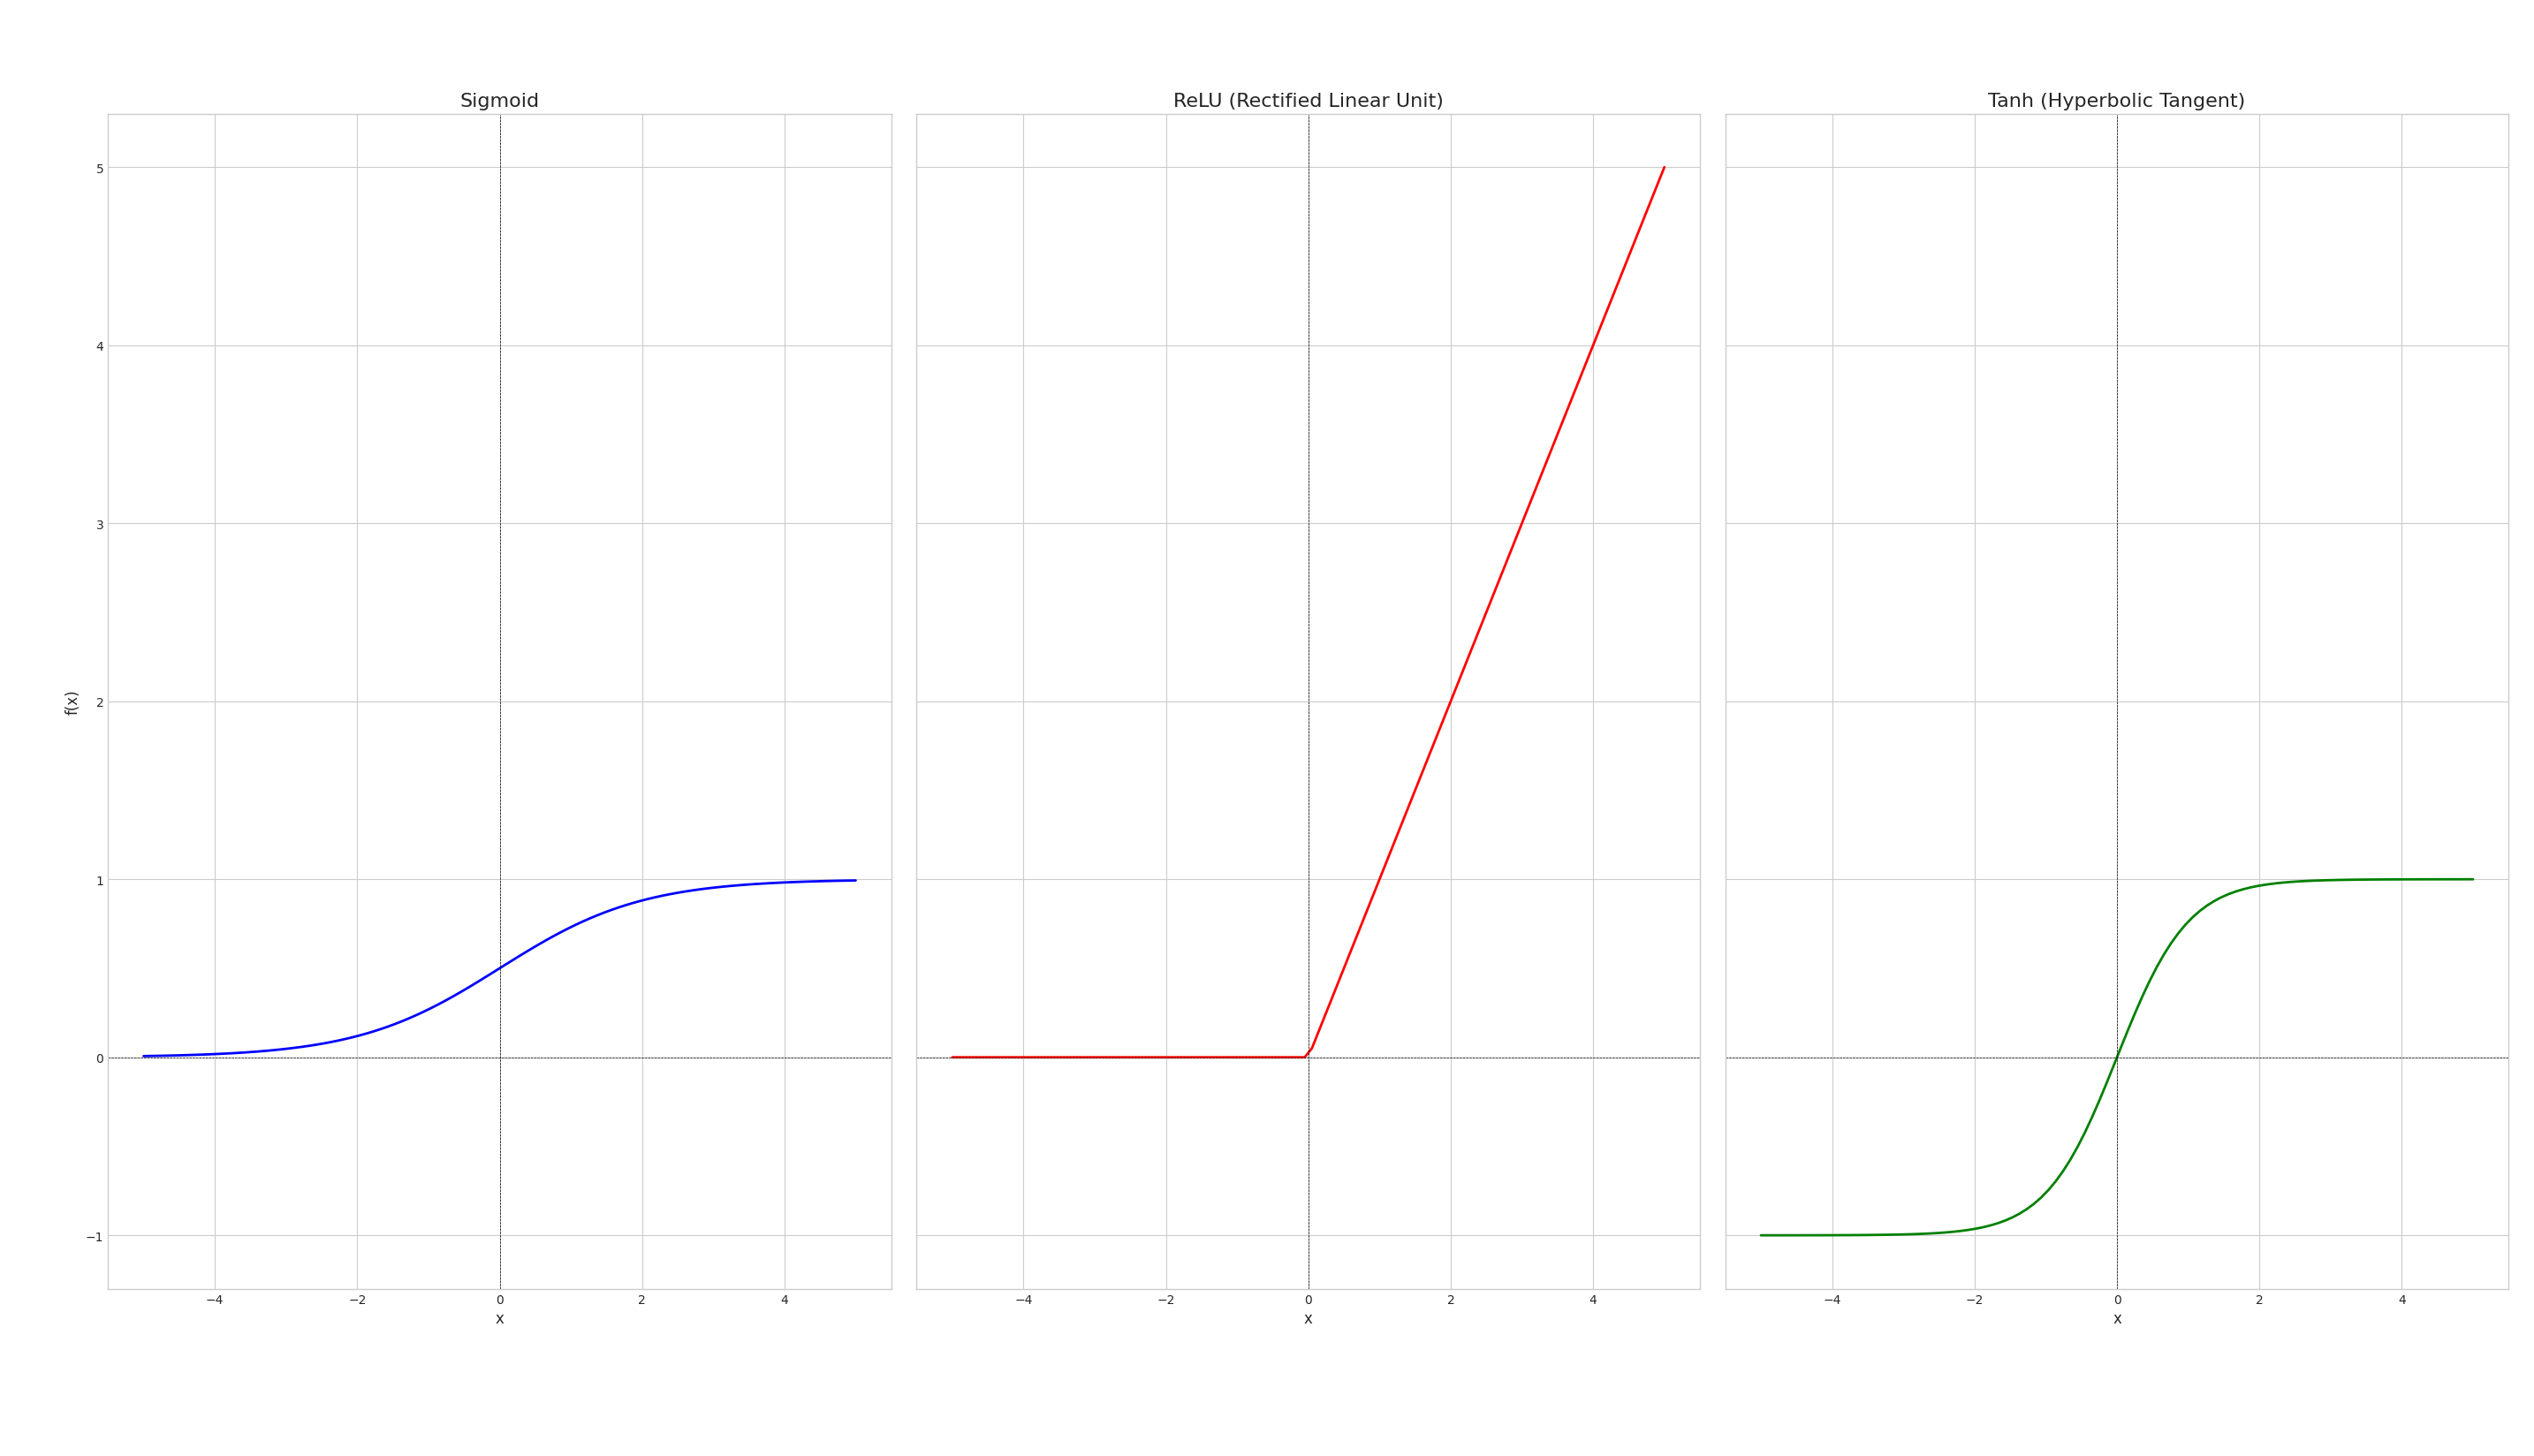
\includegraphics[width=1\textwidth]{figuras/2-fundamentos/activationFunctions.png}
    \caption{Activation Functions Examples: Sigmoid, ReLU, and Tanh}
    \label{fig:activation_function}
    \end{figure}

    These neurals are the core components of various neural network architectures, which can be organized into layers; the input layer receives the initial data, hidden layers process the data through multiple transformations, and the output layer produces the final predictions or classifications as shown in Figure \ref{fig:neural_network_architecture}. 
    
    \newpage
    \begin{figure}
    \centering
    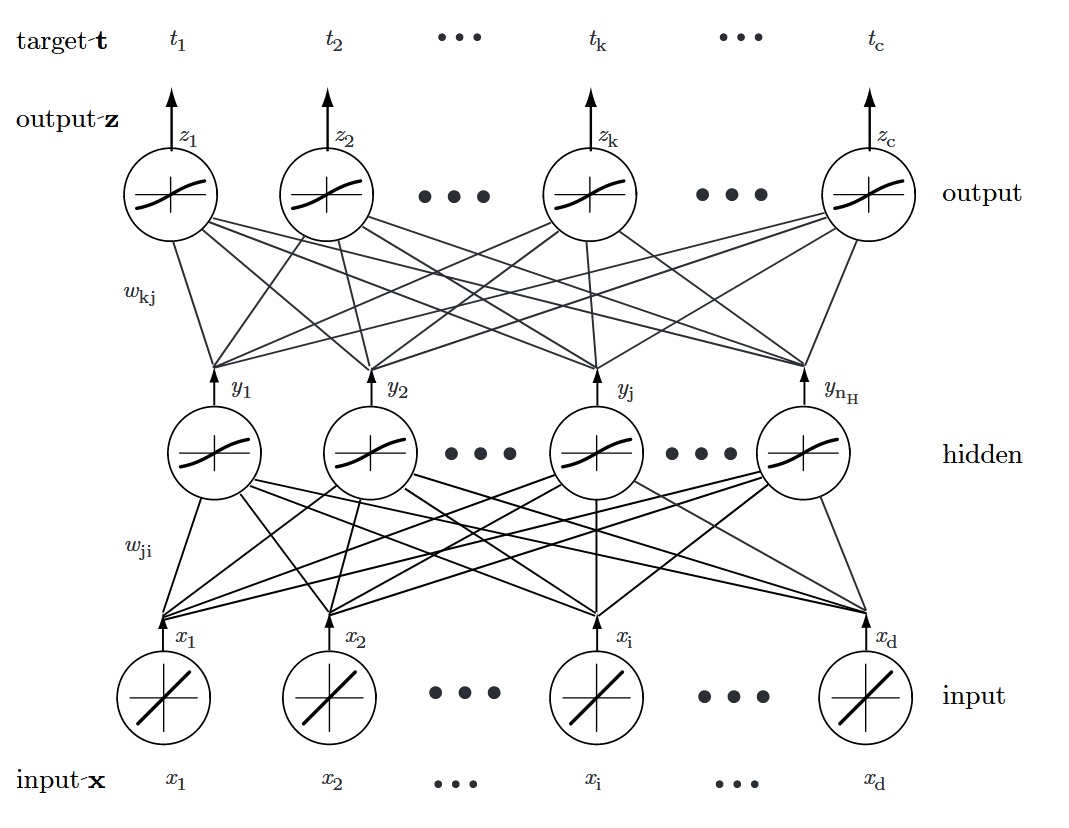
\includegraphics[width=1\textwidth]{figuras/2-fundamentos/neuralNetworkStructure.png}
    \caption{Diagram of a Neural Network with Input, Hidden, and Output Layers \cite{duda2001pattern}}
    \label{fig:neural_network_architecture}
    \end{figure}

    
    
    In practice, it is more convenient to express the forward computation of an entire layer using vectorized notation:
    \begin{align}
        \mathbf{z}^{[l]} &= \mathbf{W}^{[l]} \mathbf{a}^{[l-1]} + \mathbf{b}^{[l]}, \\
        \mathbf{a}^{[l]} &= \sigma^{[l]}\left( \mathbf{z}^{[l]} \right),
        \end{align}
where $\mathbf{a}^{[0]} = \mathbf{x}$ denotes the input vector, $\mathbf{W}^{[l]} \in \mathbb{R}^{n_l \times n_{l-1}}$ is the weight matrix, $\mathbf{b}^{[l]} \in \mathbb{R}^{n_l}$ is the bias vector, and $\sigma^{[l]}(\cdot)$ is the activation function applied elementwise.

\begin{figure}[H]
    \centering
    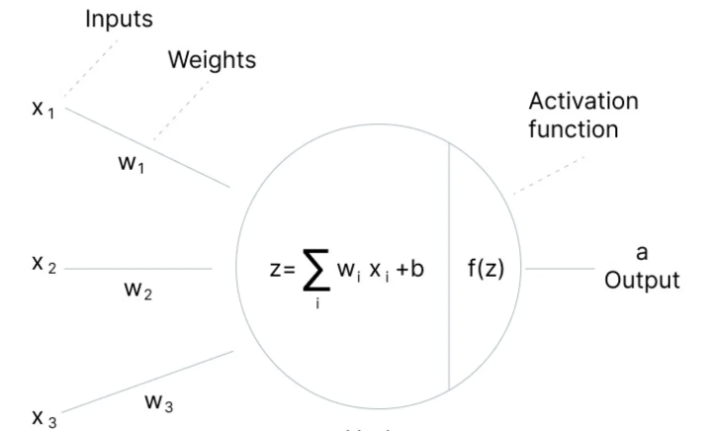
\includegraphics[width=0.8\textwidth]{figuras/2-fundamentos/neural_node.png}
    \caption{Schematic of an artificial neuron: inputs $x_i$ are weighted by $w_i$, summed with a bias $b$, and passed through a non-linear activation function $f(\cdot)$ to produce the output $y$.}
    \label{fig:neuron_diagram}
    \end{figure}

    For supervised learning tasks, the output of the final layer $\mathbf{a}^{[L]}$ is compared with the target $\mathbf{y}$ via a differentiable loss function $\mathcal{L}(\mathbf{a}^{[L]}, \mathbf{y})$. The objective of training is to minimize the cost function:
    \begin{equation}
        J(\mathbf{W}, \mathbf{b}) = \frac{1}{m} \sum_{i=1}^m \mathcal{L}\big( \mathbf{a}^{[L](i)}, \mathbf{y}^{(i)} \big),
        \end{equation}
where $m$ is the number of training samples. This minimization requires computing the gradients of $J$ with respect to each parameter $\mathbf{W}^{[l]}$ and $\mathbf{b}^{[l]}$. 

A naive computation of these gradients is computationally expensive due to the network's layered structure. The breakthrough of the backpropagation algorithm \cite{rumelhart1986learning} was to exploit the chain rule of calculus in a systematic way, allowing gradients to be propagated efficiently from the output layer back through the hidden layers. This efficiency reduced the computational cost to a scale proportional to that of the forward pass, making it feasible to train networks with many layers and large numbers of parameters.

Today, neural networks — and backpropagation in particular — form the foundation of deep learning systems used in diverse domains such as computer vision \cite{lecun1998gradient}, natural language processing \cite{vaswani2017attention}, and embedded AI for robotics and IoT \cite{lane2017squeezing}. Their adaptability to different architectures, from convolutional neural networks (CNNs) to transformers, underscores the enduring relevance of the concepts introduced more than four decades ago.


\begin{comment}
\subsection{Neural Network Architecture}

The architecture of a neural network is composed of layers of interconnected neurons. Each neuron receives inputs, applies a weighted sum followed by an activation function, and produces an output that is passed to the next layer of neurons. 

The basic building block of a neural network is the artificial neuron, which can be mathematically represented as follows:

\begin{equation}
    y = f\left(\sum_{i=1}^{n} w_i x_i + b\right)
    \end{equation}
    
    where \(y\) is the output, \(w_i\) are the weights, \(x_i\) are the inputs, \(b\) is the bias, and \(f\) is the activation function. The activation function introduces non-linearity into the model, allowing it to learn complex relationships in the data.
    
    Or visually as shown in Figure \ref{fig:neuron_diagram}, where the inputs are multiplied by their corresponding weights, summed up, and then passed through an activation function to produce the output.
    
    \newpage
    
    \begin{figure}
    \centering
    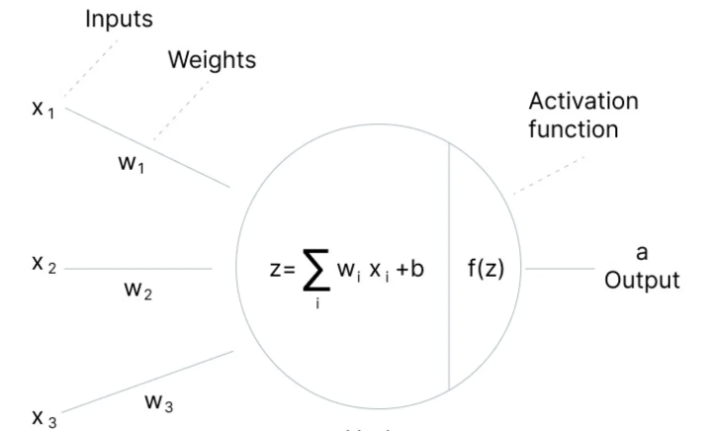
\includegraphics[width=0.8\textwidth]{figuras/2-fundamentos/neural_node.png}
    \caption{Diagram of a Single Neuron \cite{neural_node_pic}}
    
    \label{fig:neuron_diagram}
    \end{figure}
    
    Neural networks can be organized into various topologies, with the most common being Feedforward Neural Networks (FNN) and Multi-Layer Perceptrons (MLP)\cite{goodfellow2016deep}. FNNs consist of an input layer, one or more hidden layers, and an output layer, where information flows in one direction. MLPs are a specific type of FNN that includes multiple layers of neurons, allowing for more complex representations.
    
    Convolutional Neural Networks (CNNs) are another important architecture, particularly in computer vision tasks. They utilize convolutional layers to automatically learn spatial hierarchies of features from images, making them highly effective for image classification and object detection.
    
    
    % 3. Training Process
    % 3.1. Supervised Learning
    % Concept of labeled data

% Dataset split (training, validation, test)

% 3.2. Loss Functions
% MSE, Cross-Entropy (brief mention)

% 3.3. Optimization
% Gradient descent and variants (SGD, Adam)
\subsection{Training Process}
The training process of neural networks typically involves supervised learning, where the model learns from labeled data. The dataset is usually split into three parts: training, validation, and test sets. The training set is used to train the model, the validation set helps tune parameters, and the test set evaluates the model's performance on unseen data.

Loss functions are crucial in training, as they quantify the difference between the predicted outputs and the actual
labels. Common loss functions include Mean Squared Error (MSE) for regression tasks and Cross-Entropy for classification tasks shown respectively in Equations \ref{eq:mse} and \ref{eq:cross_entropy}. The choice of loss function depends on the specific task and the nature of the data.

\begin{equation}\label{eq:mse}
    \frac{1}{n} \sum_{i=1}^{n} (y_i - \hat{y}_i)^2
\end{equation}

\begin{equation}\label{eq:cross_entropy}
    -\sum_{i=1}^{n} y_i \log(\hat{y}_i)
\end{equation}

% 3.4. Backpropagation Algorithm
% How the backpropagation algorithm works
% Gradient calculation and weight updates
% Importance of backpropagation in training neural networks

These loss functions are used within backpropagation algorithm, which is the core of the training process.


% Backpropagation algorithm (brief overview or diagram)

% 4. Inference Process
% What happens when the model is deployed

% Importance of performance, size, and speed (hinting at quantization need)

% How a trained model maps input -> output

\subsubsection*{Backpropagation}
Backpropagation, short for \textit{backward propagation of errors}, is the fundamental algorithm for training artificial neural networks, enabling the efficient computation of gradients of a loss function with respect to the network’s parameters \cite{rumelhart1986learning}. It leverages the chain rule of calculus to propagate errors from the output layer back to earlier layers, systematically adjusting the weights and biases to minimize prediction error. The method was popularized in the mid-1980s, although its theoretical underpinnings can be traced back to earlier works in control theory and automatic differentiation \cite{werbos1974beyond}. Today, it remains the backbone of most supervised deep learning frameworks, being used in conjunction with optimizers such as stochastic gradient descent (SGD) and Adam.

The process begins with a \emph{forward pass}, in which the input vector $x \in \mathbb{R}^{n_0}$ is propagated layer by layer through the network. For a feedforward architecture with $L$ layers, each layer $l \in \{1, \dots, L\}$ computes a pre-activation vector $z^{[l]}$ and an activation vector $a^{[l]}$ according to
\begin{equation}
z^{[l]} = W^{[l]} a^{[l-1]} + b^{[l]}, \quad a^{[l]} = \sigma^{[l]}(z^{[l]}),
\end{equation}
where $W^{[l]} \in \mathbb{R}^{n_l \times n_{l-1}}$ is the weight matrix, $b^{[l]} \in \mathbb{R}^{n_l}$ is the bias vector, and $\sigma^{[l]}(\cdot)$ is a differentiable activation function such as the sigmoid, hyperbolic tangent, or ReLU. The input layer is given by $a^{[0]} = x$, and the network output is $\hat{y} = a^{[L]}$. The discrepancy between $\hat{y}$ and the target $y$ is measured by a differentiable loss function $\mathcal{L}(\hat{y}, y)$, and the cost over a batch of $m$ samples is
\begin{equation}
    J(W,b) = \frac{1}{m} \sum_{i=1}^{m} \mathcal{L}\big(a^{[L](i)}, y^{(i)}\big).
\end{equation}

Once the forward pass has produced the output, the \emph{backward pass} applies the chain rule to determine how a small change in each parameter affects the loss. At the output layer, the error signal is computed as
\begin{equation}
\delta^{[L]} = \nabla_a \mathcal{L}\big(a^{[L]}, y\big) \odot \sigma'^{[L]}\big(z^{[L]}\big),
\end{equation}
where $\odot$ denotes elementwise multiplication. For each preceding hidden layer $l = L-1, \dots, 1$, the error term is propagated backwards as
\begin{equation}
\delta^{[l]} = \big(W^{[l+1]}\big)^{T} \delta^{[l+1]} \odot \sigma'^{[l]}\big(z^{[l]}\big),
\end{equation}
effectively applying the chain rule to relate the sensitivity of the cost to parameters in earlier layers. Given these $\delta$ terms, the gradients with respect to the parameters are
\begin{align}
\frac{\partial J}{\partial W^{[l]}} &= \frac{1}{m} \delta^{[l]} \big(a^{[l-1]}\big)^{T}, \\
\frac{\partial J}{\partial b^{[l]}} &= \frac{1}{m} \sum_{i=1}^m \delta^{[l](i)}.
\end{align}
Finally, the parameters are updated via gradient descent,
\begin{align}
W^{[l]} &\gets W^{[l]} - \eta \frac{\partial J}{\partial W^{[l]}}, \\
b^{[l]} &\gets b^{[l]} - \eta \frac{\partial J}{\partial b^{[l]}},
\end{align}
where $\eta > 0$ is the learning rate.

The efficiency of backpropagation arises from its reuse of intermediate computations from the forward pass, avoiding redundant derivative calculations. In fact, its computational complexity is $\mathcal{O}(n)$ in the number of parameters, making it feasible for networks with millions of weights. This property, combined with the ability to use vectorized matrix operations, has made it the method of choice for modern GPUs and TPUs \cite{goodfellow2016deep}.

A high-level pseudocode for the algorithm is shown in Algorithm~\ref{alg:backprop}, where the vectorized formulation is used for batch processing. An illustration of the flow of information during forward and backward passes is provided in Figure~\ref{fig:backprop_flow}, which should be replaced with a network diagram showing activations $a^{[l]}$, pre-activations $z^{[l]}$, and gradients $\delta^{[l]}$.

\begin{figure}[H]
\centering
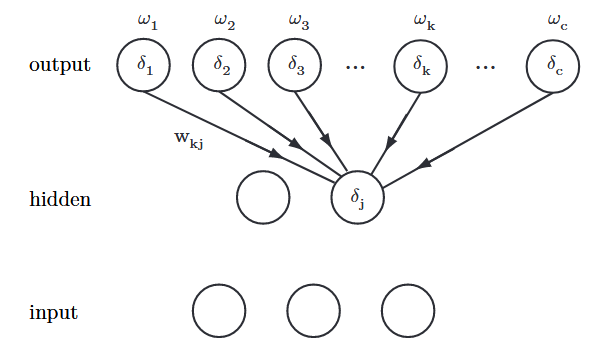
\includegraphics[width=0.85\linewidth]{figuras/2-fundamentos/backpropagation_flow.png}
\caption{Placeholder: Forward (left) and backward (right) propagation in a feedforward neural network \cite{duda2001pattern}}
\label{fig:backprop_flow}
\end{figure}

\begin{algorithm}[H]
\caption{Vectorized Backpropagation for a Fully Connected Neural Network}
\label{alg:backprop}
\begin{algorithmic}[1]
\Require Training data $\{(x^{(i)}, y^{(i)})\}_{i=1}^m$, learning rate $\eta$, number of layers $L$
\State Initialize $W^{[l]}, b^{[l]}$ for $l = 1, \dots, L$
\While{stopping criterion not met}
\State \textbf{Forward Pass:}
\State $A^{[0]} \gets X$
\For{$l = 1$ to $L$}
\State $Z^{[l]} \gets W^{[l]} A^{[l-1]} + b^{[l]}$
\State $A^{[l]} \gets \sigma^{[l]}(Z^{[l]})$
\EndFor
\State Compute cost $J$
\State \textbf{Backward Pass:}
\State $\Delta^{[L]} \gets \nabla_A \mathcal{L}(A^{[L]}, Y) \odot \sigma'^{[L]}(Z^{[L]})$
\For{$l = L-1$ down to $1$}
\State $\Delta^{[l]} \gets (W^{[l+1]})^T \Delta^{[l+1]} \odot \sigma'^{[l]}(Z^{[l]})$
\EndFor
\State \textbf{Parameter Updates:}
\For{$l = 1$ to $L$}
\State $W^{[l]} \gets W^{[l]} - \eta \frac{1}{m} \Delta^{[l]} (A^{[l-1]})^T$
\State $b^{[l]} \gets b^{[l]} - \eta \frac{1}{m} \sum_{i=1}^m \Delta^{[l](i)}$
\EndFor
\EndWhile
\end{algorithmic}
\end{algorithm}

From a theoretical standpoint, backpropagation can be interpreted as a special case of reverse-mode automatic differentiation, optimized for layered computational graphs. It assumes differentiable activation functions and loss functions, and its performance may degrade in very deep networks due to the vanishing and exploding gradient problems \cite{hochreiter1998vanishing}. Solutions such as careful weight initialization, normalization layers, and activation function design (e.g., ReLU, Leaky ReLU, GELU) have been developed to mitigate these issues.

In conclusion, backpropagation is the mathematical and computational framework that enables neural networks to learn from data by efficiently computing gradients through the chain rule. Its elegance lies in its generality: once the forward computation of a network is defined, the backward computation follows mechanically, allowing it to adapt seamlessly to a wide range of architectures, from simple perceptrons to modern transformers \cite{goodfellow2016deep}.

\end{comment}

During inference, the trained model is deployed to make predictions on new, unseen data. The performance, size, and speed of the model are critical factors in this process, especially in resource-constrained environments such as embedded systems and edge devices. The trained model maps input data to output predictions by applying the learned weights and biases through the network's layers.


% 5. Challenges and Motivations for Compression
% Overparameterization

% Memory usage

% Latency

% Deployment on microcontrollers, edge devices

\subsection{Challenges and Motivations for Compression}
Despite their effectiveness, NN face several challenges, specially Overparameterization, which may lead to a significant increase of memory usage and a higher latency during inference process \cite{han2015deepcompression}. These challenges become particularly pronounce when deploying models of embbeded systems, where the resource is limited. One common solution to address these challenges is quantization, which reduces the precision of the model, leading to a faster inference and lower memory usage. 



\section{Quantization}

%1.1 Definition and Basic Idea
%General concept: reducing the precision of data by mapping continuous or high-precision values to a smaller set of fixed levels.

Quantization is a model compression technique aimed at reducing the numerical precision of neural network parameters and activations, thereby lowering both memory usage and computational cost \cite{jacob2018quantization,han2016deep}. The core idea is to map continuous or high-precision values to a smaller discrete set of representable levels. This approach, widely used in signal processing and image compression, has proven effective for deploying deep learning models on resource-constrained devices such as mobile phones and microcontrollers.

Mathematically, given a real-valued matrix of activations or weights $\mathbf{A} \in \mathbb{R}^{m \times p}$ and a target bit-width $n$, the quantization operator $Q$ can be defined as:
\begin{equation}
Q(n, \mathbf{A}) = \text{clip}\left( \text{round}\left(\frac{\mathbf{A}}{q(\mathbf{A}, n)}\right)-Z,\ -2^{n-1},\ 2^{n-1}-1 \right),
\label{eq:quantization}
\end{equation}
where $q(\mathbf{A}, n)$ is the scaling factor, $\text{round}(\cdot)$ rounds to the nearest integer, $\text{clip}(\cdot)$ restricts values to the range $[-2^{n-1}, 2^{n-1}-1]$ and $Z$ is an integer zero point.

The scaling factor $q(\mathbf{A}, n)$ partitions the dynamic range of $\mathbf{A}$ into $2^n$ equally spaced levels:
\begin{equation}
q(\mathbf{A}, n) = \frac{\beta - \alpha}{2^n - 1},
\label{eq:scaling}
\end{equation}
where $\alpha = \min(\mathbf{A})$ and $\beta = \max(\mathbf{A})$. The dequantization step reconstructs an approximation $\hat{\mathbf{A}}$ of the original values:
\begin{equation}
\hat{\mathbf{A}} = q(\mathbf{A}, n) \cdot Q(n, \mathbf{A}).
\label{eq:dequantization}
\end{equation}

Figures~\ref{fig:quant_n1} and \ref{fig:quant_n2} illustrate uniform quantization for $n=1$ and $n=2$, respectively, showing the effect of reducing the representable precision.
\begin{figure}[H]
    \centering
    \begin{minipage}{0.48\textwidth}
        \centering
        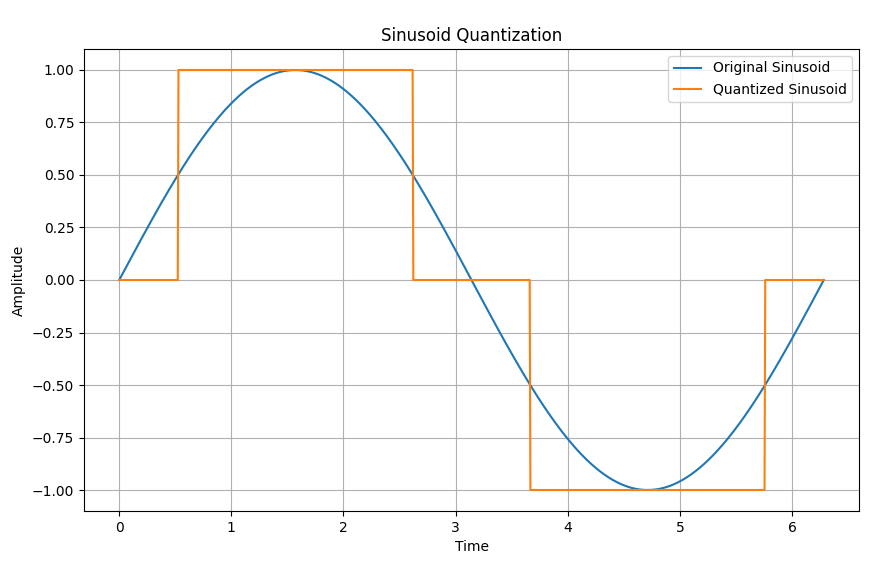
\includegraphics[width=0.75\linewidth]{figuras/2-fundamentos/quantization_n=1.png}
        \caption{Uniform quantization with $n=1$.}
        \label{fig:quant_n1}
    \end{minipage}
    \hfill
    \begin{minipage}{0.48\textwidth}
        \centering
        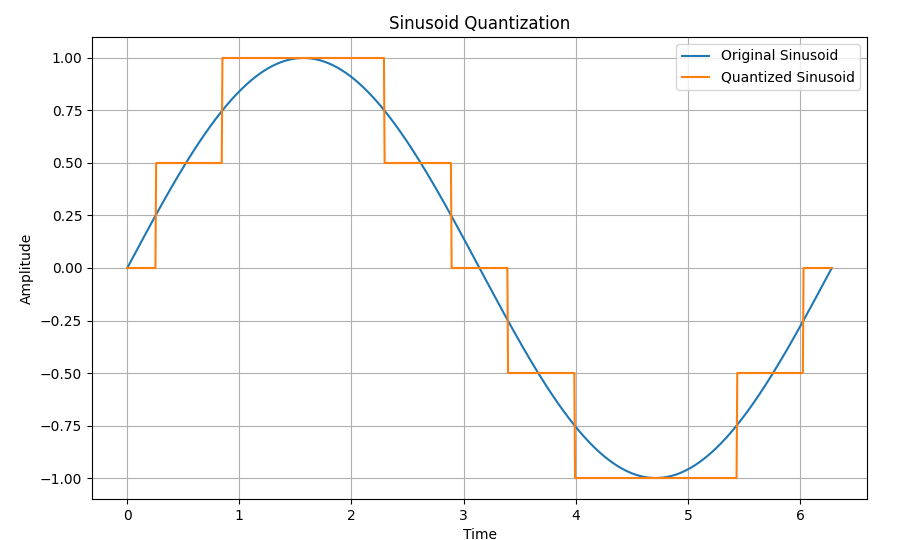
\includegraphics[width=0.75\linewidth]{figuras/2-fundamentos/quantization_n=2.png}
        \caption{Uniform quantization with $n=2$.}
        \label{fig:quant_n2}
    \end{minipage}
\end{figure}

\subsubsection*{Symetric vs. Asymmetric Quantization}
Quantization strategies also can be classified into symmetric and asymetric quantization. In sysmetric quantization, the zero-point is set to zero, and the scaling factor is applied uniformly across the entire range of values, i.e., $\alpha = -\beta$. This approach is simpler and often sufficient for many applications, especially when the distribution of values is approximately centered around zero.

\newpage
\begin{figure}
\centering
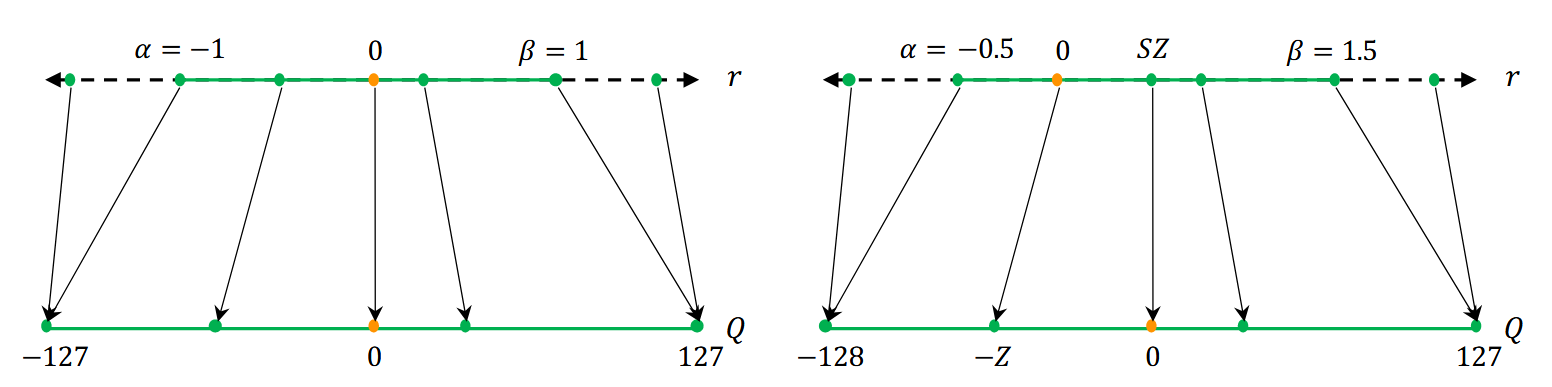
\includegraphics[width=0.8\textwidth]{figuras/2-fundamentos/quantization symetric.png}
\caption{Symetric and asymetric quantization.}
\label{fig:symmetric_quantization}
\end{figure}


Quantization strategies can be categorized as:
\begin{itemize}
    \item \textbf{Uniform vs. Non-uniform:} Uniform quantization uses equally spaced levels, while non-uniform methods allocate more levels to ranges with higher probability density.
    \item \textbf{Symetric vs. Asymmetric:} Symmetric quantization has a zero point at zero, while asymmetric quantization allows for a non-zero zero point, which can better fit unbalanced distributions.
    \item \textbf{Layer-wise vs. Channel-wise:} Layer-wise quantization applies a single quantization scheme to all parameters in a layer, while channel-wise quantization applies different schemes to each channel or filter, allowing for more flexibility and potentially better accuracy.
    \item \textbf{Fixed-point vs. Floating-point:} Fixed-point formats are more hardware-friendly and power-efficient, whereas low-bit floating-point formats (e.g., FP16, bfloat16) preserve a wider dynamic range.
\end{itemize}


The most important aspect of quantization to our scope would be the representation of fixed-point numbers and floating-point numbers. Floating-point quantization, also called as fake quantization, is a techique that simulates the effects of quantization during training, allowing the model to adapt and be represented in low precision formats, but still mainting the floating-point representation \cite{Zhu2020Survey}. It, therefore, requires the hardware to perform calculations in floating-point format, which is more flexible but less efficient than fixed-point arithmetic.

Fixed-point quantization represents numbers with a fixed number of bits for the integer and fractional parts, allowing for faster arithmetic operations and lower memory usage. This representation is particularly suitable for resource-constrained devices, where computational efficiency is crucial.

\subsection{ANN Quantization}

Strategies to quantize ANN are numerous and with many combinations of techiniques \cite{jacob2018quantization, Zhu2020Survey}. The choice of strategy depends on the specific application, hardware constraints, and desired trade-offs between accuracy and efficiency. For the sake of this work, we will focus on the quantization of weights, activations functions and biases, which are the most common components to be quantized in ANN.

In general, we could use the equation \ref{eq:quantization} to quantize the weights, activations and biases of a neural network. The quantization of the weights is performed layer by layer, where each layer $l$ has its own bit-width $n_l$:

\begin{equation}
W^{[l],q} = Q(n_l, W^{[l]}) \quad \text{for } l = 1, \dots, L,
\end{equation}
where $n_l$ is the bit-width for the $l$-th layer. The quantization of the biases follows a similar approach:
\begin{equation}
b^{[l],q} = Q(n_l, b^{[l]}) \quad \text{for } l = 1, \dots, L.
\end{equation}

However, there a considerations that must be taken into account when mapping each neural network element to the quantized representation. 

\subsubsection*{Weights}

Within uniform quantization, weights can be quantized using symmetric or asymmetric schemes \cite{Zhu2020Survey}. Symmetric quantization is widely adopted for weights because it simplifies the quantization function by setting the zero point ($Z$) to zero \cite{Zhu2020Survey}. This results in a simpler quantization function \ref{eq:quantization}, which reduces computational cost during inference and makes implementation more straightforward. In such cases, the clipping range is symmetric around zero, often chosen based on the maximum absolute value of the weights. The "full range" approach (e.g., [-128, 127] for 8 bits) is generally more accurate than the "restricted range" (e.g., [-127, 127]) \cite{Zhu2020Survey}. On the other hand, asymmetric quantization uses a clipping range that is not necessarily symmetric and is preferred when weight distributions are unbalanced, as it can result in a tighter clipping range and better utilization of available bit width.

The granularity of weight quantization is another critical factor. 
\begin{itemize} 
    \item Layerwise quantization applies a single clipping range to all weights within a layer. While simple to implement, it often results in sub-optimal accuracy if the range of individual convolutional filters varies widely. 
    \item Groupwise quantization groups multiple channels within a layer to calculate the clipping range. This can be useful when parameter distributions vary significantly within a convolution but incurs an additional cost to account for different scaling factors. 
    \item Channelwise quantization is the standard method for quantizing convolutional kernels. It assigns a dedicated scaling factor to each convolutional filter, ensuring better quantization resolution and often resulting in higher accuracy with negligible overhead. 
    \item Sub-channelwise quantization offers the most granular control, but adds considerable overhead due to managing multiple scaling factors, making it less common. 
\end{itemize}

Integer-only quantization, which is more desirable than simulated quantization. This is because all operations are performed using low-precision integer arithmetic \cite{Zhu2020Survey}, which fully leverages low-precision hardware logic, which is faster, more power-efficient, and more area-efficient.

To mitigate post-quantization accuracy degradation, fine-tuning methods are employed. Quantization Aware Training (QAT) involves re-training the model with quantized parameters so that it can converge to a point with better loss and recover accuracy \cite{Zhu2020Survey} QAT can also learn optimal quantization parameters, such as clipping ranges and scaling factors for weights, during training. However, its main disadvantage is the high computational cost due to extensive re-training. An alternative is Post-Training Quantization (PTQ), which quantizes and adjusts weights without any re-training, offering a very low and often negligible overhead \cite{Zhu2020Survey}. While faster, PTQ generally results in lower accuracy compared to QAT \cite{Zhu2020Survey}. For scenarios where no training/validation data is accessible, Zero-Shot Quantization (ZSQ) methods are used. 

\begin{comment}
    
    Finally, to mitigate significant accuracy degradation in low-precision scenarios, mixed-precision quantization is utilized [62: \cite{Zhu2020Survey}; 65: \cite{Zhu2020Survey}]. This approach applies different bit precisions to different layers of the model [58: \cite{Zhu2020Survey}; 62: \cite{Zhu2020Survey}], with more sensitive layers kept at higher precision and less sensitive layers at lower precision [65: \cite{Zhu2020Survey}; 87: \cite{Zhu2020Survey}]. This aims to balance accuracy and efficiency across the model, minimizing accuracy degradation while still benefiting from reduced memory footprint and acceleration [65: \cite{Zhu2020Survey}]. Determining the optimal bit allocation per layer can involve complex search problems, such as reinforcement learning-based methods or Hessian-aware techniques [63: \cite{Zhu2020Survey}; 64: \cite{Zhu2020Survey}]. This approach has proven hardware-efficient, showing significant accelerations compared to uniform precision quantization [64: \cite{Zhu2020Survey}; 65: \cite{Zhu2020Survey}].
\end{comment}


\subsubsection*{Bias}



While the literautre sources does not outline a single, standard quantization method for biases, there is a large discussion mainly focussed on correction techniques \cite{Zhu2020Survey}. 


A known consequence of certain approuches, such as PTQ can lead to a shift in the mean of the weight and activation values, a factor that negatively impacts model accuracy. The solution lies in applying bias correction method that seek to readjust these deviations \cite{Zhu2020Survey}.

The choice between symmetric and asymmetric quantization directly influences this dynamic. In asymmetric quantization, where the clipping range is not necessarily centered at the origin, cross-terms emerge. As these terms are static, they can be absorbed by the layer's bias, which represents a practical optimization in hardware implementation. In contrast, symmetric quantization is inherently free of this issue, as its zero-centered range does not generate such terms.

Beyond these considerations, other techniques focus on making the neural network more amenable to quantization. Range Equalization, for example, normalizes the value ranges of weights across layers, which implicitly standardizes the activations and reduces overall error. The efficacy of this approach is amplified in Zero-Shot Quantization scenarios, where the absence of calibration data makes bias error correction a fundamental step. Indeed, the most robust solutions for quantizing without training data often integrate both weight equalization and bias correction, creating a synergy that preserves the robustness of the quantized model.

\subsubsection*{Activations}

To quantize activations it depends on the activation function used in ANN. For instance, ReLU activations are typically quantized using symmetric quantization, while other activation functions may require asymmetric quantization. The quantization of activations is performed layer by layer, where each layer $l$ has its own bit-width $n_l$:
\begin{equation}
A^{[l],q} = Q(n_l, A^{[l]}) \quad \text{for } l = 1, \dots, L,
\end{equation}



\section{Neural Network Equivalence}

In the context of NN, equivalence refers to the property that two neural networks can produce the same outputs given the same set of inputs. This is particularly important when considering the quantization process, where the goal is to reduce the network's size to fit NN into a resource-constrained environment without significantly degrading its performance.
In this section, we will define the equivalence of neural networks and the assumptions that must be satisfied to ensure that the quantized neural network (QNN) is equivalent to the original floating-point neural network (FNN).

We define the equivalence of neural networks in terms of their outputs for a given input space. Specifically, we consider two neural networks, $f$ and $t$, where $f$ is the original floating-point neural network and $t$ is the quantized neural network. The equivalence condition can be expressed as follows:
\begin{equation}
f(x) \sim t(x), \quad \forall x \in I,
\end{equation}
where $I$ is the input space and $O$ is the output space. This means that for every input $x$ in the input space, the output of the original neural network $f$ and the output of the quantized neural network $t$ must produce the same class label or output value.

\subsection{Types of Equivalence in Neural Networks}

There are two distict ways to measure similarity between two neural networks: \textbf{similar representation} and \textbf{similar function}. Similar representation means that the two neural networks have the same structure, i.e., the same number of layers, the same number of neurons in each layer, and the same activation functions. Similar function means that the two neural networks produce the same output for the same input.

To our scope, we will focus on the second definition, which is more relevant to the quantization process.

Similar function means that the two neural networks produce the same output for the same input. 



\subsection{Formal Verification of Neural Network Equivalence}

To verify the equivalence of neural networks, we define a formal 


\textbf{Neural Networks:} $\Gamma$ and $F$ \\
\textbf{Input Space:} $I \in \mathbb{R}^n$ \\
\textbf{Output Space:} $O \in \mathbb{R}^n$ \\

\textbf{Objective:} Prove that the mathematical functions of $\Gamma$ and $F$, $f:I \rightarrow O$ and $t:I\rightarrow O$, are equivalent.

\textbf{Equivalence:} Both NNs produce the same outputs for the same inputs.

\textbf{Definition 1 (Top-1-Equivalence):} Two NNs $f$ and $t$ are Top-1-equivalent if:
$$ \arg\max f(x) = \arg\max t(x), \forall x \in I $$

\textbf{Assumption 1:} For NN $F$ without quantization:
$$ \arg\max f(x) = y, \text{ for } x \in H $$

\textbf{Assumption 2:} For NN $F$ with quantization:
$$ \exists N \text{ such that } \arg\max f(x) = \arg\max f^q(x) = y, \forall x \in H $$



\textbf{Objective:} Maximize quantization while maintaining QNN equivalence to the floating point NN.

\textbf{Definition 2 (Robust Quantization):}
Let \( f \) be the reference NN and \( H \subset \mathbb{R}^n \) be a set of instances. Robust quantization is defined as:
\[ \text{Quantization of } f \text{ resulting in } f^q \text{ such that } \arg\max f(x) \Leftrightarrow \arg\max f^q(x), \forall x \in H \]

\textbf{Quantization Assumption:}
There exists a set \( N = \{n_1, n_2, \ldots, n_L\} \), where \( n_l \in N \) represents the number of bits for quantizing the \( l \)-th layer in \( f \).

\textbf{Robust Quantization Problem:}
Obtain a sequence of \( N \) where each \( n \in N \) is minimized, ensuring the equivalence between \( f \) and \( f^q \) is satisfied.


We consider the robust quantization of a neural network (NN) as an iterative minimization problem. Each iteration consists of two complementary sub-problems:

\begin{enumerate}
  \item Minimize the quantization bit widths by finding a candidate set \( N \).
  \item Verify the equivalence property, i.e., check if an NN quantized with the bit widths in \( N \) is equivalent to the original NN.
\end{enumerate}

\textbf{If the latter fails, we iteratively return to the minimization sub-problem with additional information.}

\begin{equation}
    N^o = \arg\min_{n_1,...,n_L} \sum_{l \in N_l <= L} n_l 
\end{equation}
    
$$
\begin{aligned}
& \arg\max f(x) = \arg\max f^q(x), & \forall x \in H^o_{CE} \\
& n_l \geq \underline{N} \vee n_l  \in N^o \\
& n_l  \leq \overline{N}  \vee n_l  \in N^o 
\end{aligned}
$$
    

Consider \( \overline{N} \) to be the upper limit and \( \underline{N} \) the lower one.
\begin{itemize}
  \item \( \overline{N} \) ensures two things:
  \begin{enumerate}
    \item It gives an upper bound to the quantization bit width.
    \item It provides a termination criterion. If a candidate \( N^o \) is found such that \( n_l = \overline{N} \) for every \( n_l \in N^o \), the optimization stops as it reaches Assumption 2.
  \end{enumerate}
  \item Assumption 2 ensures the termination of CEG4N, built on the premise that there exists a set of \( N \) where quantization introduces minimal error to the NN.
  \item If CEG4N proposes a quantization solution equal to \( \overline{N} \), this solution is verified, and if verification returns a counter-example, CEG4N finishes with failure.
  \item Note that \( H^o_{CE} \) is an iterative parameter, updated at each iteration based on the verification sub-problem.
\end{itemize}

In the Verification sub-problem $o$, we check whether the $N^o$ generated by the optimization sub-problem $o$ satisfies the following equivalence property:

\[\Psi(f,f^q, x,y)=\Psi_x(x)\rightarrow \Psi_y(y)\]

if  $\Psi_x(x)\rightarrow \Psi_y(y)$ holds for the candidate $N^o$, the optimization halts and $N^o$ is declared as solution; otherwise, a new counter-example $H_{CE}$ is generated. Iteration o+1 starts where iteration o stopped. That is, the optimization sub-problem o + 1 receives as parameter a set of $H^{+1}_{CE}$ such that $H^{o+1}_{CE}=H^o_{CE}\cup x_{CE}$.

\begin{comment}
    
    \subsection{Problem Encoding}
    
    \subsection{Neural Network Equivalence Problem}
    
    
    \subsection{Network Repair}
    
    Like said before, QNN are widely employed in human-activity. However, the quantization process can lead to a significant loss of accuracy. To address this issue, researchers have explored various techniques to repair quantized neural networks (QNNs).
    
    Repair NN have two main objectives: fix defects found in Neural Networks. It can be classified into three categories: retraining/fine-tuning, direct weight modification, and architecture extension \cite{song2023qnnrepair}.
    
    The equivalence problem is a fundamental challenge in the field of neural Network Repair. It shows that the equivalence problem can be reduced to a Satisfiability problem \cite{eleftheriadis2022neuralnetworkequivalencechecking}.
    
    
    
    
    \textcolor{red}
    {This approuch is not exclusive to QNNs.}
    
    \begin{itemize}
    \item AIREPAIR: A Repair Platform for Neural Networks
\end{itemize}

Reluplex: An Efficient SMT Solver for Verifying  Deep Neural Networks?

- This paper does not deal with quantized neural network
- Deep Neural Networks (DNN)
- It has been discovered that DNN can be disturbed even by the slighest pertubation
- Verifying DNN is a difficult problem. They are large, non-linear, and non convex.
- It's a NP-COMPLETE problem.
- LP Solvers and SMT solvers can be employed to verify DNN but until now have only be used to verify small Models.
- Activation function are a problem because they are non linear, thus the papers focus only in Relu
- It found out that some of RELU during search can be ignored.

Contribution
- Reluplex presents itself as a SMT solver for a theory of real time arithmetic with ReLu constrains

\end{comment}

\chapter{Methodology} \label{chap:metodologia}

\begin{figure}
\centering
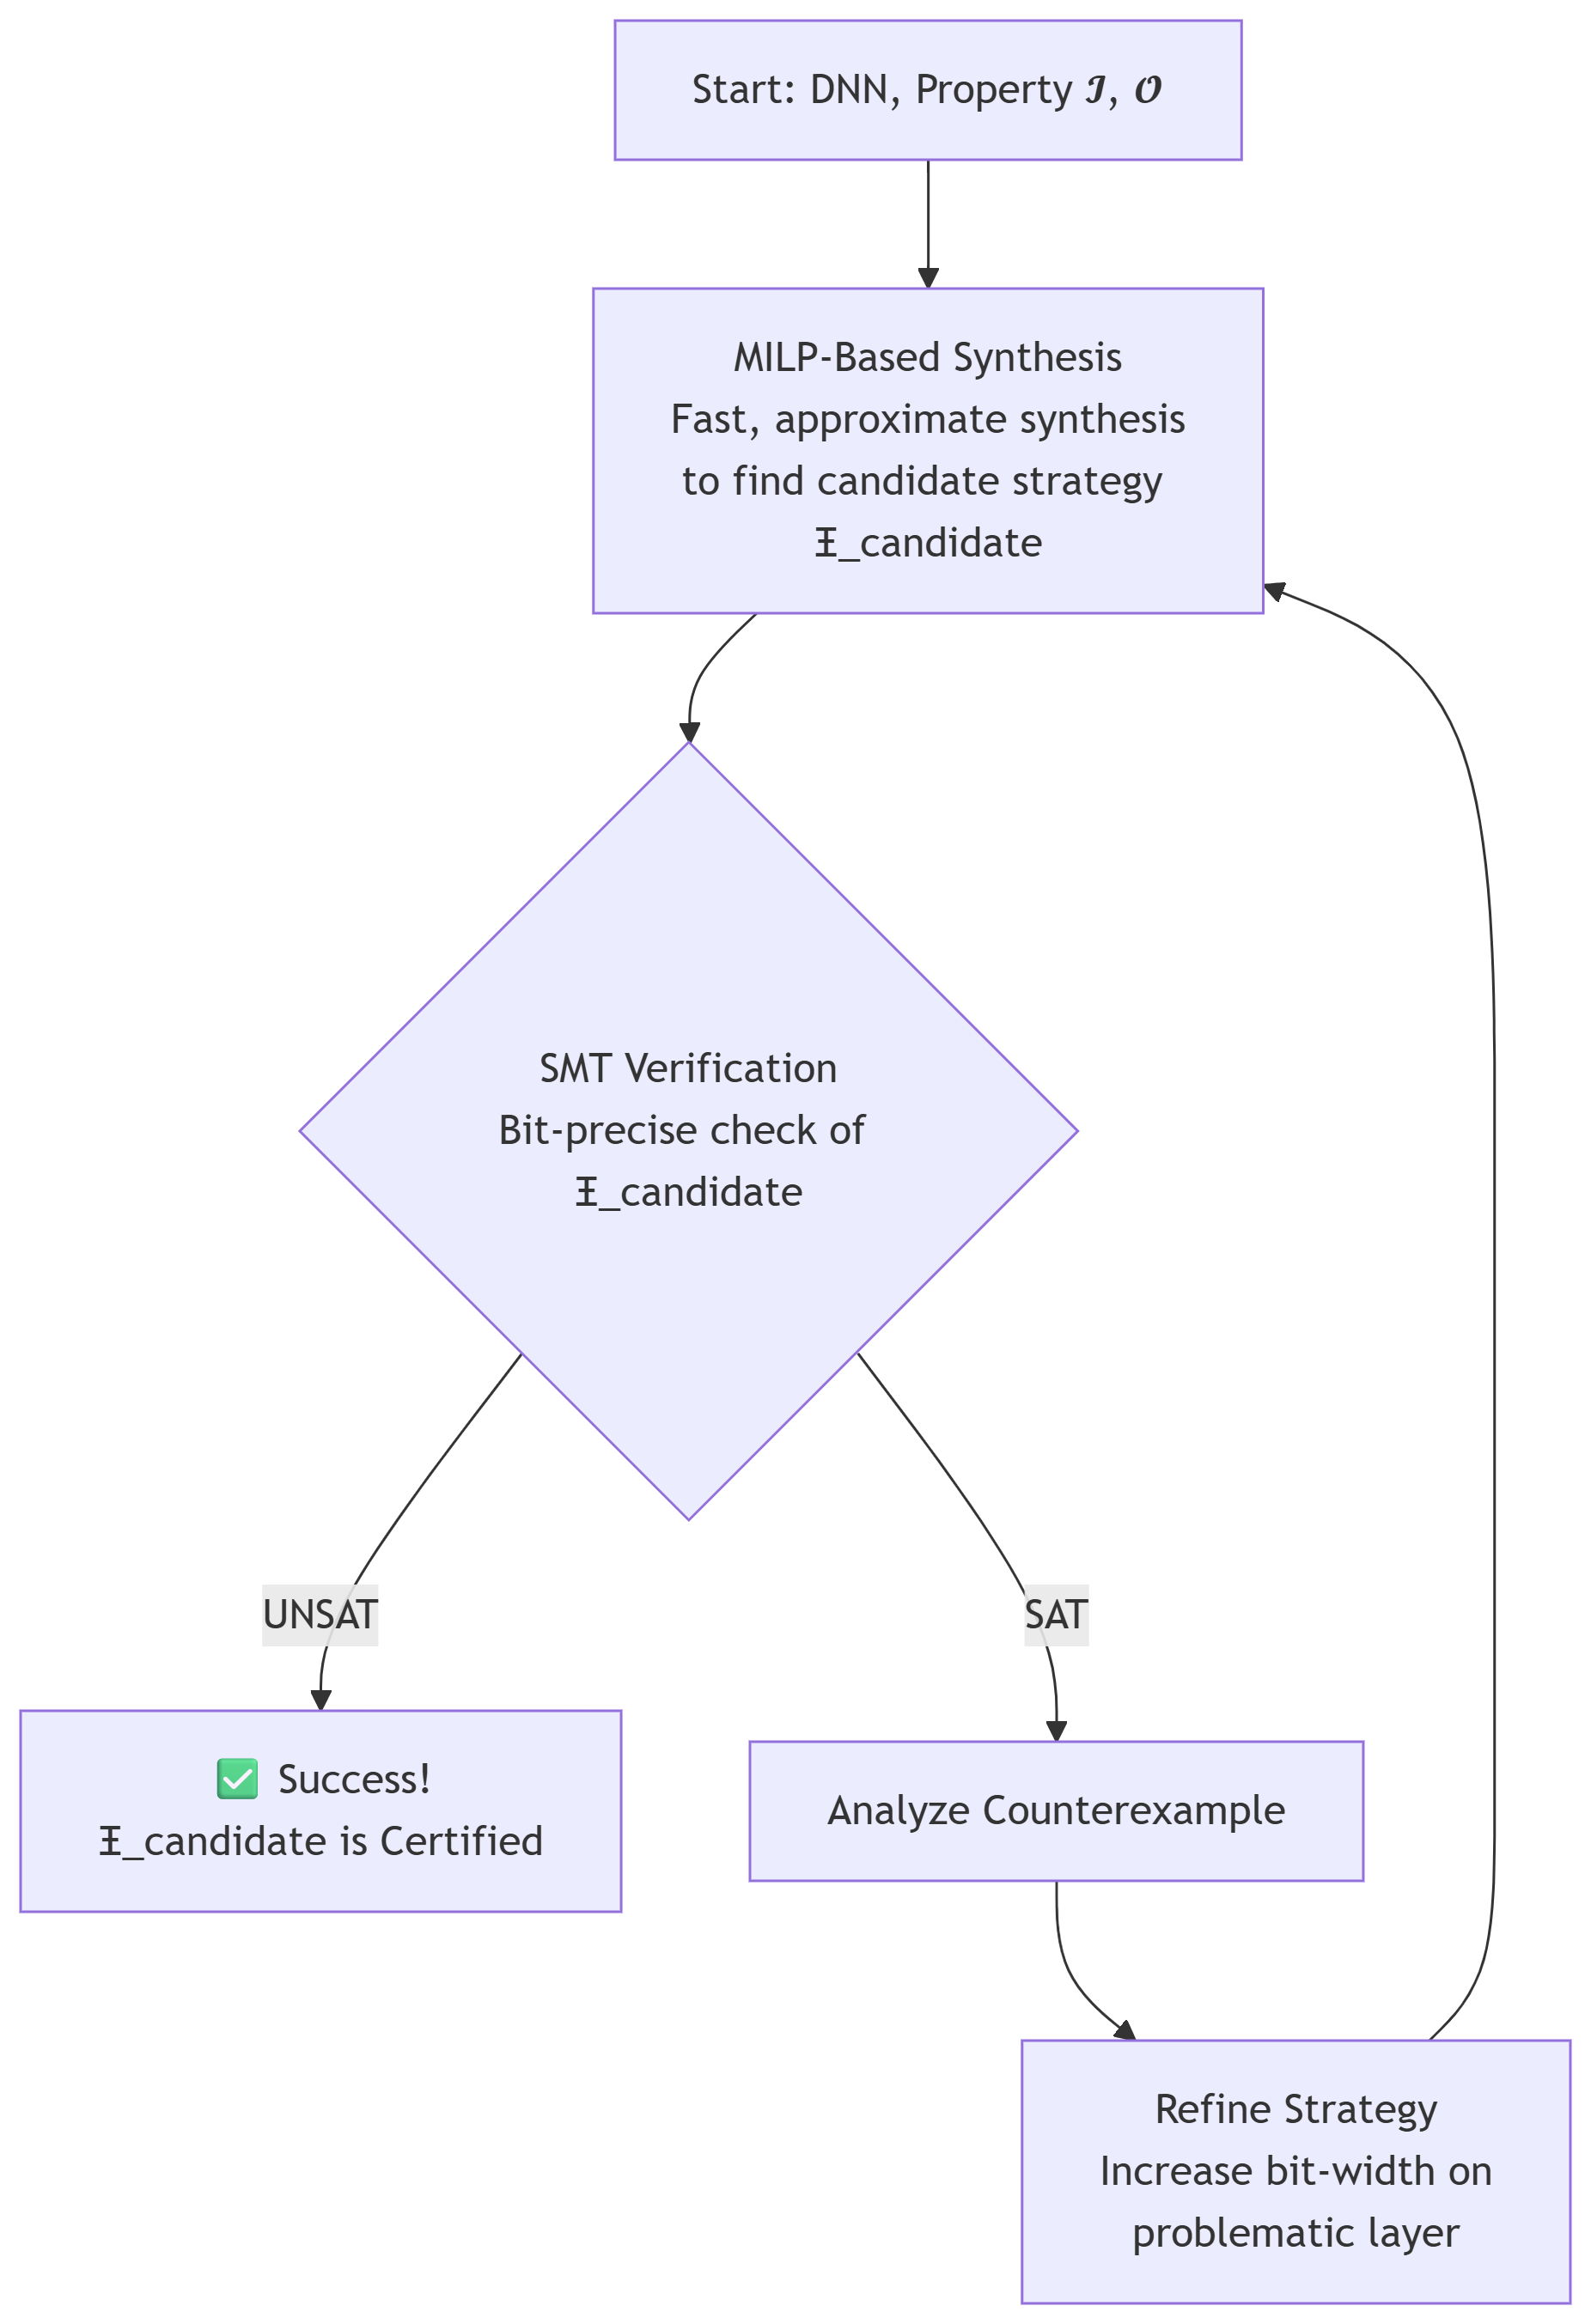
\includegraphics[width=0.3\textwidth]{figuras/3-metodologia/frameworkDiagram.png}
\caption{\textcolor{red}{(POSSIBLE DIAGRAM)}}
\label{fig:frameworkDiagram}
\end{figure}
\newpage
\section{Problem}

ANN are widely used in various applications, but their computational and memory resource demands are high \cite{amir2021smt, han2020understanding, abdi2021counterexample, song2023qnnrepair}. Quantization is a crucial technique to mitigate this problem by reducing the bit-width (from 32-bit floating-point to 8-bit integers or even binary) used to represent weights, biases, and activations, making networks more efficient on embedded and low-power devices \cite{amir2021smt, han2020understanding,song2023qnnrepair, abdi2021counterexample, Cai2020Certified}.

However, quantization introduces an "implementation gap" \cite{cordeiro2025neuralnetworkverificationprogramming}. Most formal verification techniques for neural networks (such as Reluplex and Marabou) assume that networks operate with real-number arithmetic \cite{katz2017reluplex,amir2021smt}. In contrast, actual hardware implementations use finite-precision arithmetic, such as low-precision floating-point or, more frequently, fixed-point \cite{han2020understanding}. This discrepancy means that the safety and correctness guarantees obtained on ideal models may not hold for the deployed neural network \cite{abdi2021counterexample}.

Furthermore, quantization, while beneficial for efficiency, can degrade accuracy and, more critically, compromise desired safety and correctness properties, such as adversarial robustness (resistance to small input perturbations that change the classification) and the absence of backdoors (intentionally inserted vulnerabilities). Existing work on QNN verification generally focuses on post-hoc analyses; that is, they verify a network after it has been quantized \cite{abdi2021counterexample,Cai2020Certified}.

\section{Proposed Approach}

\textcolor{red}{Poderias inserir um diagrama para apresentar a sua metodologia? A partir desse diagrama, você pode descrever cada bloco da metodologia por seções.}

This dissertation proposes the development of a framework for the certified synthesis of quantization strategies that guarantee the preservation of desired properties after quantization, directly addressing finite-precision arithmetic. This differs from post-hoc approaches and quantization techniques that focus solely on accuracy.

\textbf{Synthesis of Quantization Strategies (Inspired by Quadapter):}
The work Quadapter is the first to propose the synthesis of certified quantization strategies \cite{Zhu2021Quadapter,Cai2020Certified}. Its central idea is to compute the pre-image of each layer concerning the desired output region and then identify the minimum bit-width for each layer, ensuring that the quantized layer's reachable region remains within that pre-image.

This dissertation would extend this line of work by focusing on the incorporation of fixed-precision arithmetic during the synthesis process. This is not the primary focus of Quadapter in its current state, which, while dealing with realistic quantization representations, does not yet formally incorporate the nuances of fixed-point arithmetic during verification.

\textbf{Formal Integration of the SMT Theory of Fixed-Point Arithmetic:}
A fundamental contribution would be the use of the SMT Theory of Fixed-Point Arithmetic, as formalized by \cite{baranowski2020smt}. This theory provides a rigorous formalization for fixed-point operations, including rounding modes (roundUp, roundDown) and overflow modes (saturation, wrapAround).

The proposal is to integrate this formal theory into the pre-image calculation and quantization procedures of the synthesis framework. This would allow the synthesized quantization strategies to be certified for the specific finite precision of the hardware, ensuring that properties hold even with the effects of rounding and overflow. The methods of \cite{baranowski2020smt} already include decision procedures for this theory, via both bit-vectors and reals, which is essential for a verifier. They present a case study that utilizes this theory to validate QNNs.

This would more robustly solve the "implementation gap," as the formal guarantees would be directly on the behavior of fixed-point arithmetic, not just a real-number approximation.

\textbf{Pre-image Calculation with Fixed-Point Semantics:}
Quadapter uses a method based on Mixed-Integer Linear Programming (MILP) to compute under-approximations of the pre-image. This dissertation would adapt this MILP formulation to precisely reflect fixed-point operations (including rounding and overflow) instead of just real numbers. This would ensure that the calculated pre-image already accounts for the effects of finite precision.

\textbf{Bit-Precise Verification in Progressive Quantization:}
In Quadapter's progressive quantization algorithm, the verification step $\left(\gamma(\hat{A}_{2i}) \subseteq P_{2i}\right)$ \textcolor{red}{(Still have to add the math theory)} compares the quantized reachable region with the pre-image. The proposal is to use formal SMT-based fixed-point reasoning (potentially through backends like ESBMC) to perform this verification in a bit-precise manner \cite{esbmc2025}. This would mean that the inclusion of the quantized reachable region within the pre-image would be verified considering the exact rules of fixed-point arithmetic.

QNN verification is a PSPACE-hard problem, and scalability is a known challenge for all verifiers (e.g., Marabou, Reluplex, CEG4N). Even Quadapter faces timeouts in pre-image calculations \cite{cai2025certified}.

\textbf{Adaptive/Dynamic Quantization:} While Quadapter synthesizes per-layer bit-widths, this research could explore how to fine-tune precision (e.g., different precisions within a layer, as discussed by \cite{han2020understanding,abdi2021counterexample}) in a verification-guided manner to minimize bit requirements without losing properties, seeking a balance that optimizes verifier performance.

\section{Experimental Methodology}

To empirically validate the certified quantization synthesis methodology proposed in this dissertation, a meticulous selection of public benchmarks, widely recognized in the formal verification of neural networks community, will be used. The choice of benchmarks was designed to ensure a comprehensive evaluation, covering a variety of network architectures, application domains, and safety properties. The basis for this selection includes the challenges proposed by the Neural Network Verification Competition (VNN-COMP) and the test suites made available in foundational works in the field \cite{cordeiro2025neuralnetworkverificationprogramming,abdi2021counterexample}.

The evaluation suite will be composed of the following main components. First, for image classification tasks, we will use models trained on the \textbf{MNIST}, \textbf{CIFAR-10}, and \textbf{Fashion-MNIST} datasets. These range from simple, few-layer networks, ideal for scalability analysis, to complex architectures like LeNet, VGGNet, ResNet-18, and MobileNetV2, allowing the framework to be evaluated in realistic scenarios \cite{han2020understanding, qnsong2023qnnrepairCai2020Certified}. Second, for the domain of safety-critical systems, the \textbf{ACAS Xu} benchmark will be central, given its status as the de facto standard for verifying airborne controllers \cite{katz2017reluplex}. Finally, to enable agile prototyping and debugging, smaller-scale models will be employed, such as those used in the \textbf{fairness} case studies with tabular data and the fixed-point quantized \textbf{Cart-Pole} controller \cite{baranowski2020smt}. The primary focus of the certified synthesis will be the preservation of \textbf{adversarial robustness}, a critical and extensively studied property, with the possibility of extension to other formal specifications.


\section{Expected Contributions}
An innovative framework and methodology for the certified synthesis of bit-precise quantization strategies for neural networks, offering formal guarantees that extend to finite-precision implementations.

A formal and empirical demonstration of the impact of fixed-point arithmetic semantics on the preservation of properties during quantization.

Significant scalability improvements for the verification and synthesis of larger and deeper QNNs by combining the power of SMT with fixed-point theory and optimization techniques.

An extension of the approach to guarantee other critical properties, such as adversarial robustness and the absence of backdoors, beyond the functional equivalence already explored in different contexts (e.g., CEG4N) \cite{abdi2021counterexample}.

This dissertation would fill a critical gap in the research, providing a rigorous foundation for the deployment of safe and reliable neural networks in resource-constrained critical systems.




%\input{capitulos/4-resultados}
%\input{capitulos/5-conclusão}

%% Referencias
%\backmatter %turns off chapter numbering and doesn't fiddle with page numbering
%\nocite{*} % mostra todas as referencias disponiveis, se estiver comentado mostra apenas referências citadas ao longo do texto
%\bibliographystyle{cls_bst/bst_ufam}
% Troca o estilo para (author, ano)
\bibliographystyle{apalike}
\bibliography{referencias}

%% apêndice
\appendix
\chapter{Artigos Publicados}
Neste apêndice, o artigo desenvolvido nesta dissertação é apresentado.


\end{document}
